\documentclass[11pt, a4paper]{article}
\usepackage[margin=1in]{geometry}
\usepackage[T1]{fontenc}
\usepackage{lmodern}
\usepackage{microtype}
\usepackage{booktabs}
\usepackage{tabularx}
\usepackage{amsmath, amssymb}
\usepackage{enumitem}
\usepackage{xcolor}
\usepackage{hyperref}
\usepackage{float}
\usepackage{caption}
\usepackage{subcaption}
\usepackage{multirow}
\usepackage{graphicx}

\graphicspath{{figures/}}

\definecolor{accentblue}{HTML}{2563EB}
\definecolor{muted}{HTML}{64748B}
\definecolor{neg}{HTML}{DC2626}
\definecolor{pos}{HTML}{16A34A}

\hypersetup{
  colorlinks=true,
  linkcolor=accentblue,
  urlcolor=accentblue,
  citecolor=accentblue,
}

\setlength{\parindent}{0pt}
\setlength{\parskip}{6pt}

\usepackage{titlesec}
\titleformat{\section}{\large\bfseries\sffamily}{\thesection.}{0.5em}{}[\vspace{-4pt}\rule{\textwidth}{0.4pt}]
\titleformat{\subsection}{\normalsize\bfseries\sffamily}{\thesubsection}{0.5em}{}
\titleformat{\subsubsection}{\normalsize\itshape}{\thesubsubsection}{0.5em}{}

\title{%
  \sffamily\bfseries
  Annexure~1: Isometric Projection Experiment\\[4pt]
  \Large Effect of Physically Correct Z-Scaling on\\
  VLM-Based Embryo Stage Classification
}
\author{%
  Gently Project, Shroff Lab, Janelia Research Campus
}
\date{March 2026}

\begin{document}
\maketitle

\begin{abstract}
We test whether physically correct (isometric) Z-scaling in orthogonal
projections improves VLM-based developmental stage classification.  The diSPIM
microscope produces anisotropic voxels: $Z = 1.0\;\mu\text{m}$,
$XY = 0.1625\;\mu\text{m/pixel}$ (6.15:1 ratio).  Standard three-view
projections compress the Z axis, producing visually flattened side and front
views.  We hypothesized that correcting this distortion---rescaling Z to match
XY---would give the model more accurate depth information and improve
classification.

The result is unambiguously negative.  Isometric projections reduce exact
accuracy by 7.8--14.8 percentage points across two prompt variants, with
adjacent accuracy dropping by 11.1--16.1 percentage points.  Analysis of the
confusion matrices reveals that isometric Z-scaling amplifies inter-specimen
morphological variation relative to inter-stage variation, causing the model to
match embryos by individual shape rather than developmental stage.
\end{abstract}

% ═══════════════════════════════════════════════════════════════
\section{Motivation}
% ═══════════════════════════════════════════════════════════════

The three-view orthogonal projection is the primary image representation sent
to Claude for stage classification.  It composites three max-intensity
projections---XY (top-down), YZ (side), and XZ (front)---into a single image.

The diSPIM imaging system has highly anisotropic voxels:

\begin{center}
\begin{tabular}{@{}lrl@{}}
\toprule
\textbf{Axis} & \textbf{Resolution} & \textbf{Source} \\
\midrule
$X$, $Y$ (lateral) & 0.1625~$\mu$m/pixel & $6.5\;\mu\text{m} / 40\times$ objective \\
$Z$ (axial)        & 1.0~$\mu$m/step     & Piezo step size \\
\midrule
$Z : XY$ ratio     & 6.15 : 1            & \\
\bottomrule
\end{tabular}
\end{center}

In the standard (non-isometric) projection, each voxel maps to one pixel
regardless of axis, so the Z dimension appears $6.15\times$ compressed.  A
side view that should span 310 pixels at correct scale renders as only 53
pixels.  This is physically inaccurate and obscures depth structure.

We hypothesized that correcting this anisotropy---rendering projections at
true physical scale---would improve stage classification by providing the model
with geometrically faithful depth information.

% ═══════════════════════════════════════════════════════════════
\section{Visual Comparison}
% ═══════════════════════════════════════════════════════════════

\subsection{Non-isometric vs.\ isometric projections across developmental stages}

Figure~\ref{fig:stages-comparison} shows the same embryo (embryo\_1) at five
developmental stages, rendered with non-isometric (top row) and isometric
(bottom row) projections.  The isometric images are substantially larger due
to the $6.15\times$ Z-axis expansion, and the side/front views (YZ and XZ)
dominate the visual field.

\begin{figure}[H]
\centering

\begin{subfigure}[t]{0.19\textwidth}
\centering
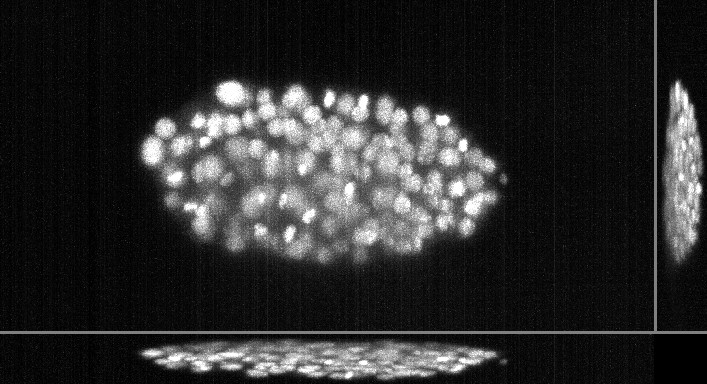
\includegraphics[width=\textwidth]{early_noniso.jpg}
\end{subfigure}
\begin{subfigure}[t]{0.19\textwidth}
\centering
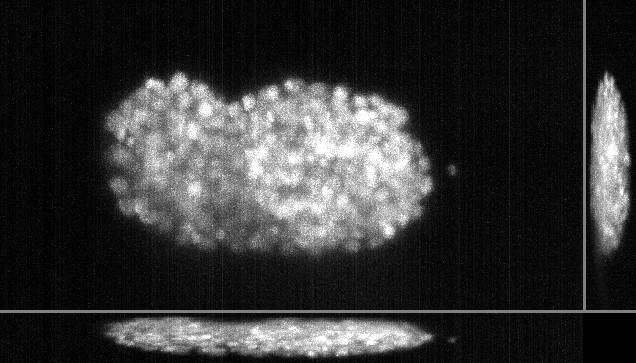
\includegraphics[width=\textwidth]{bean_noniso.jpg}
\end{subfigure}
\begin{subfigure}[t]{0.19\textwidth}
\centering
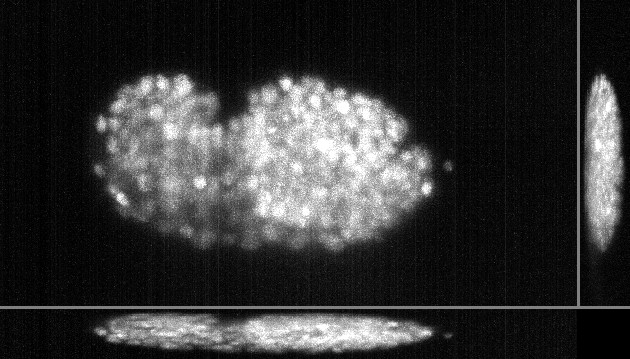
\includegraphics[width=\textwidth]{comma_noniso.jpg}
\end{subfigure}
\begin{subfigure}[t]{0.19\textwidth}
\centering
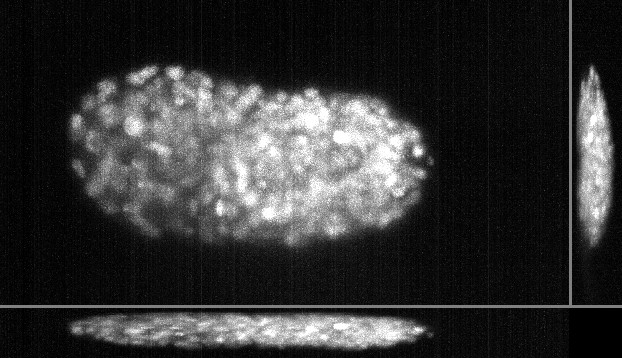
\includegraphics[width=\textwidth]{1.5fold_noniso.jpg}
\end{subfigure}
\begin{subfigure}[t]{0.19\textwidth}
\centering
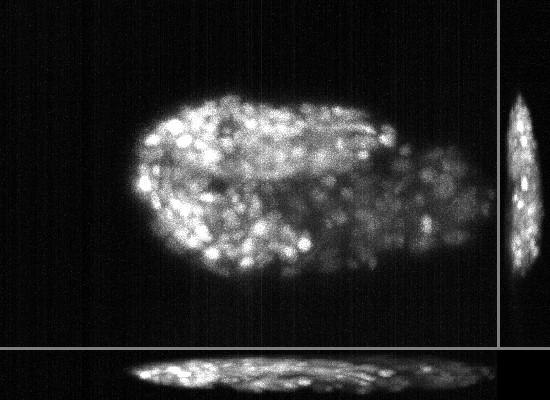
\includegraphics[width=\textwidth]{pretzel_noniso.jpg}
\end{subfigure}

\vspace{4pt}

\begin{subfigure}[t]{0.19\textwidth}
\centering
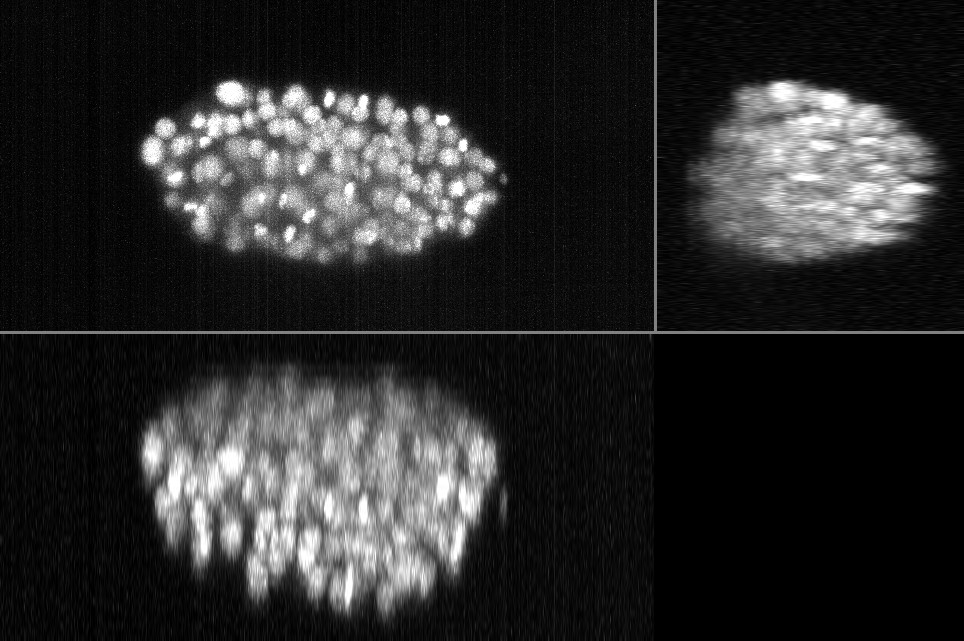
\includegraphics[width=\textwidth]{early_iso.jpg}
\caption*{Early}
\end{subfigure}
\begin{subfigure}[t]{0.19\textwidth}
\centering
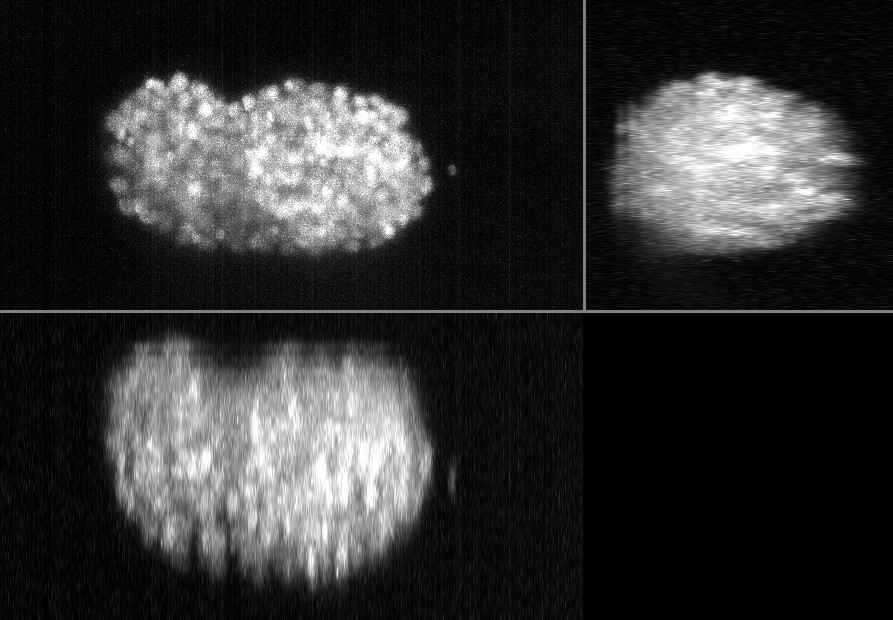
\includegraphics[width=\textwidth]{bean_iso.jpg}
\caption*{Bean}
\end{subfigure}
\begin{subfigure}[t]{0.19\textwidth}
\centering
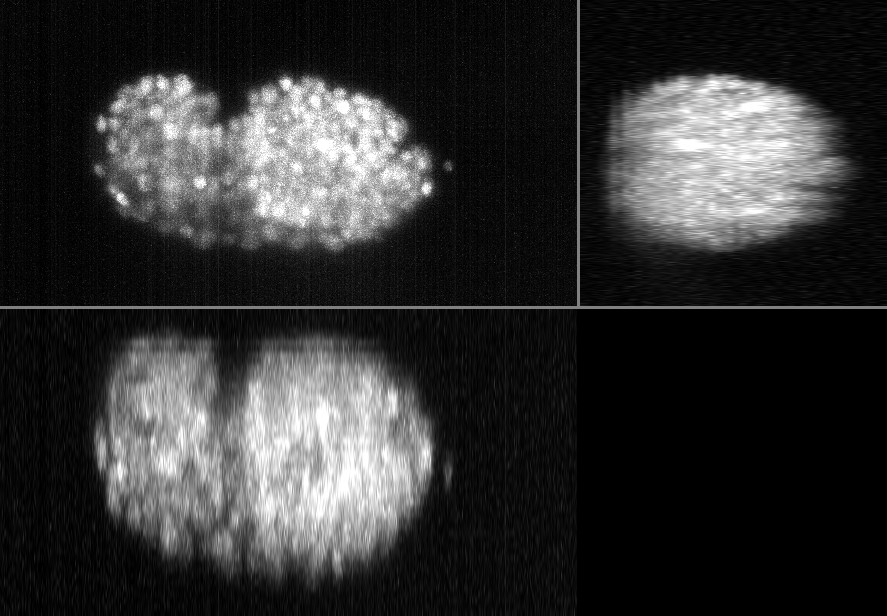
\includegraphics[width=\textwidth]{comma_iso.jpg}
\caption*{Comma}
\end{subfigure}
\begin{subfigure}[t]{0.19\textwidth}
\centering
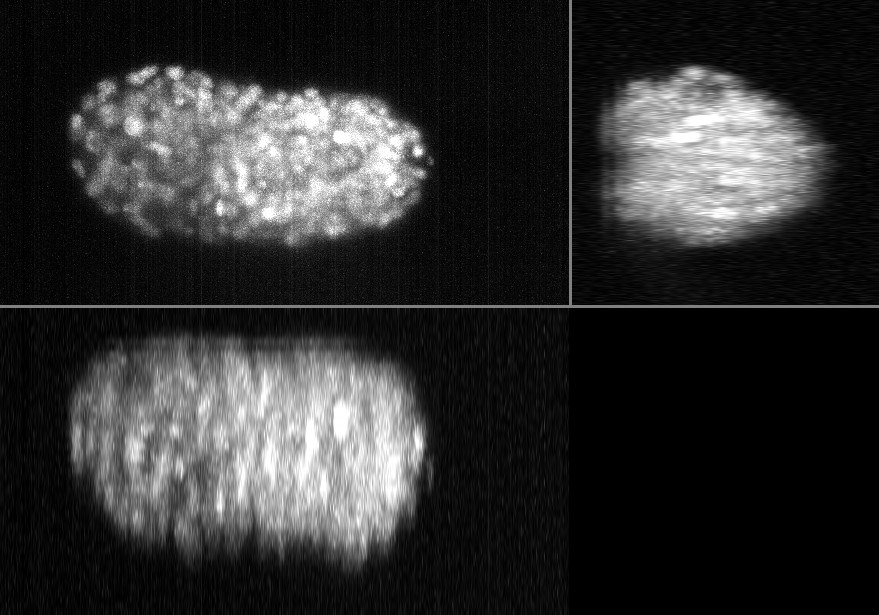
\includegraphics[width=\textwidth]{1.5fold_iso.jpg}
\caption*{1.5-fold}
\end{subfigure}
\begin{subfigure}[t]{0.19\textwidth}
\centering
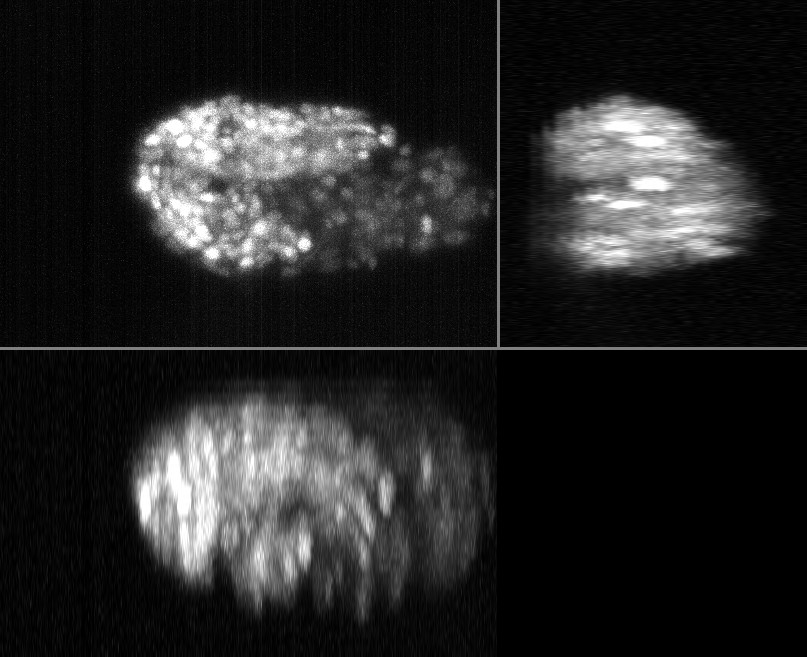
\includegraphics[width=\textwidth]{pretzel_iso.jpg}
\caption*{Pretzel}
\end{subfigure}

\caption{Non-isometric (top row) vs.\ isometric (bottom row) three-view
projections of embryo\_1 across five developmental stages.  In non-isometric
views, the XY top-down projection dominates; in isometric views, the
Z-expanded side and front views become visually prominent.}
\label{fig:stages-comparison}
\end{figure}

\subsection{Inter-embryo variation at the same stage}

Figure~\ref{fig:inter-embryo} shows all four embryos at the early stage
(T10), comparing non-isometric and isometric projections.  With non-isometric
projections, the four embryos appear broadly similar (symmetric ovals).  With
isometric projections, specimen-specific Z profiles become prominent and
visually distinctive---each embryo has a unique side/front view shape
depending on its orientation in the imaging chamber.

\begin{figure}[H]
\centering

\begin{subfigure}[t]{0.24\textwidth}
\centering
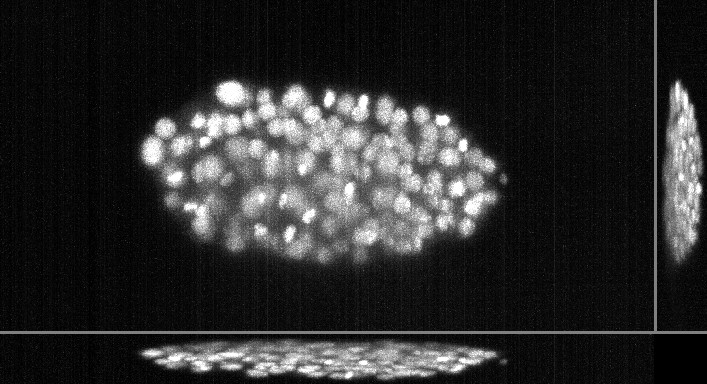
\includegraphics[width=\textwidth]{embryo_1_T10_noniso.jpg}
\end{subfigure}
\begin{subfigure}[t]{0.24\textwidth}
\centering
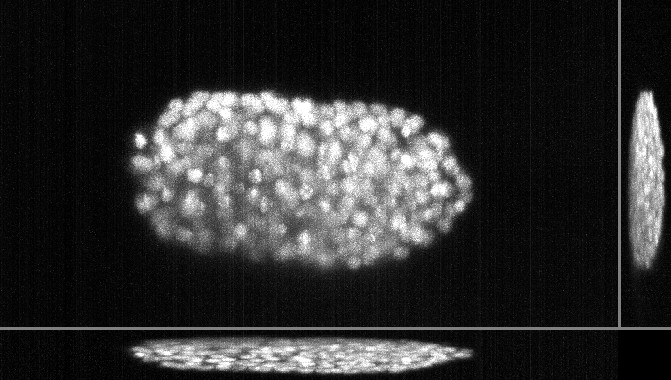
\includegraphics[width=\textwidth]{embryo_2_T10_noniso.jpg}
\end{subfigure}
\begin{subfigure}[t]{0.24\textwidth}
\centering
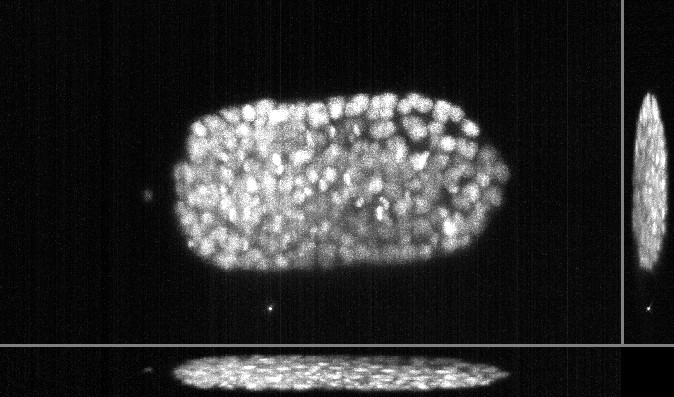
\includegraphics[width=\textwidth]{embryo_3_T10_noniso.jpg}
\end{subfigure}
\begin{subfigure}[t]{0.24\textwidth}
\centering
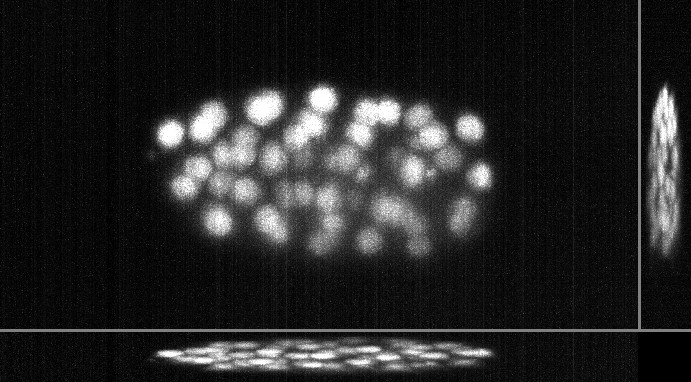
\includegraphics[width=\textwidth]{embryo_4_T10_noniso.jpg}
\end{subfigure}

\vspace{4pt}

\begin{subfigure}[t]{0.24\textwidth}
\centering
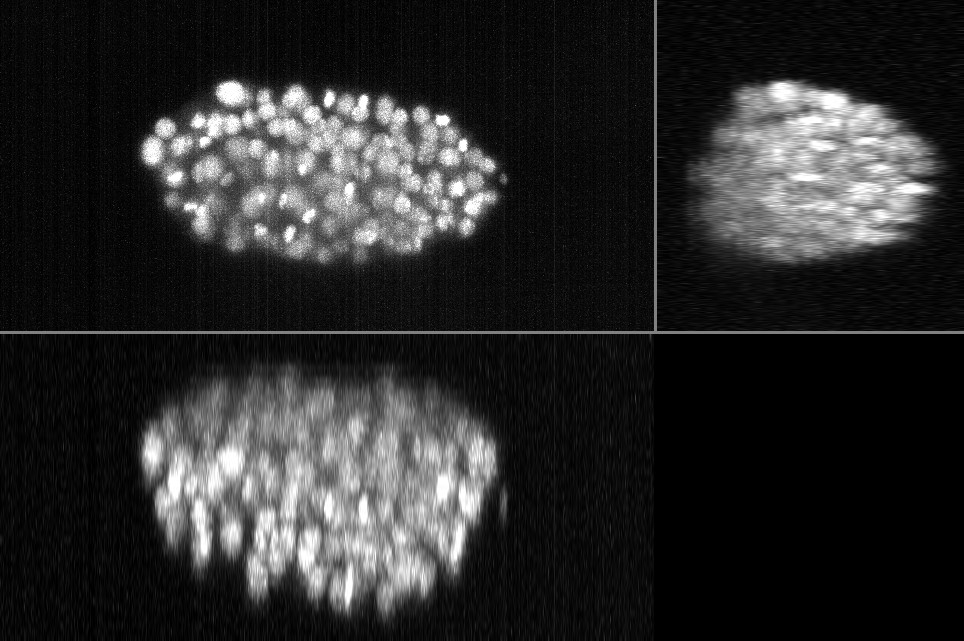
\includegraphics[width=\textwidth]{embryo_1_T10_iso.jpg}
\caption*{Embryo 1}
\end{subfigure}
\begin{subfigure}[t]{0.24\textwidth}
\centering
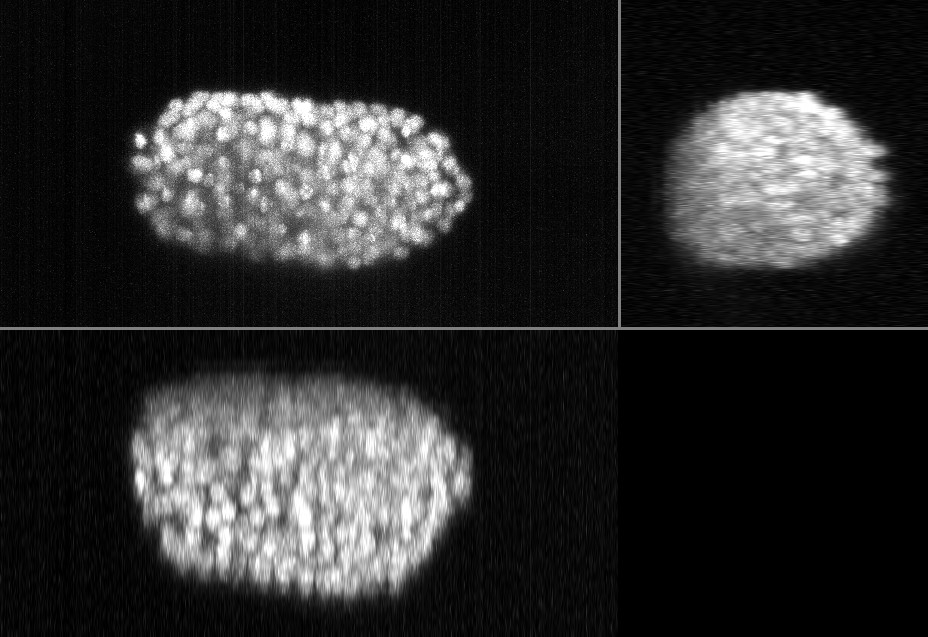
\includegraphics[width=\textwidth]{embryo_2_T10_iso.jpg}
\caption*{Embryo 2}
\end{subfigure}
\begin{subfigure}[t]{0.24\textwidth}
\centering
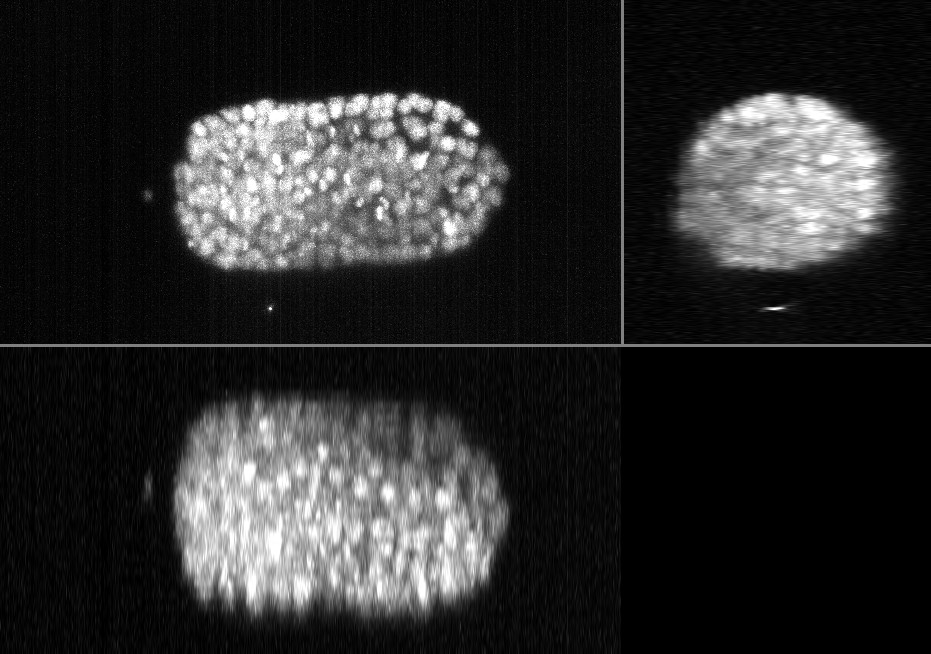
\includegraphics[width=\textwidth]{embryo_3_T10_iso.jpg}
\caption*{Embryo 3}
\end{subfigure}
\begin{subfigure}[t]{0.24\textwidth}
\centering
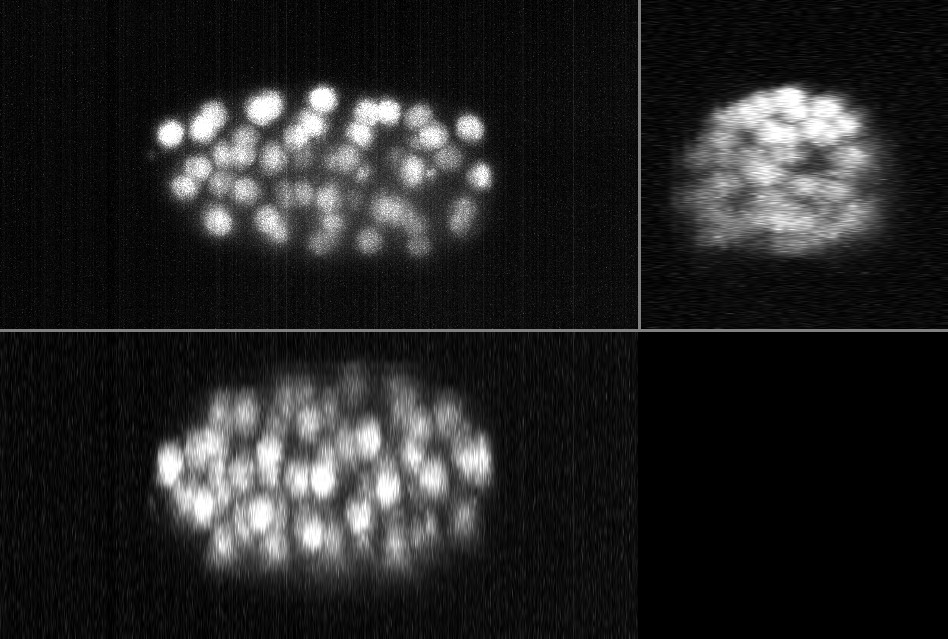
\includegraphics[width=\textwidth]{embryo_4_T10_iso.jpg}
\caption*{Embryo 4}
\end{subfigure}

\caption{Four embryos at the early stage (T10).  Non-isometric (top row) vs.\
isometric (bottom row).  Non-isometric views look similar across specimens;
isometric views expose specimen-specific Z profiles that drive misclassification.}
\label{fig:inter-embryo}
\end{figure}

\subsection{Cross-stage confusion: why embryo\_3 early looks like pretzel}

Figure~\ref{fig:confusion-case} illustrates the key failure mode.  The
reference images (from embryo\_2) define what each stage ``looks like'' to the
model.  With isometric projection, embryo\_3's early-stage Z profile happens
to resemble embryo\_2's pretzel reference more than embryo\_2's early
reference.  Conversely, embryo\_4's pretzel Z profile does not match the
pretzel reference, leading to ``early'' predictions at late stages.

\begin{figure}[H]
\centering

\begin{subfigure}[t]{0.45\textwidth}
\centering
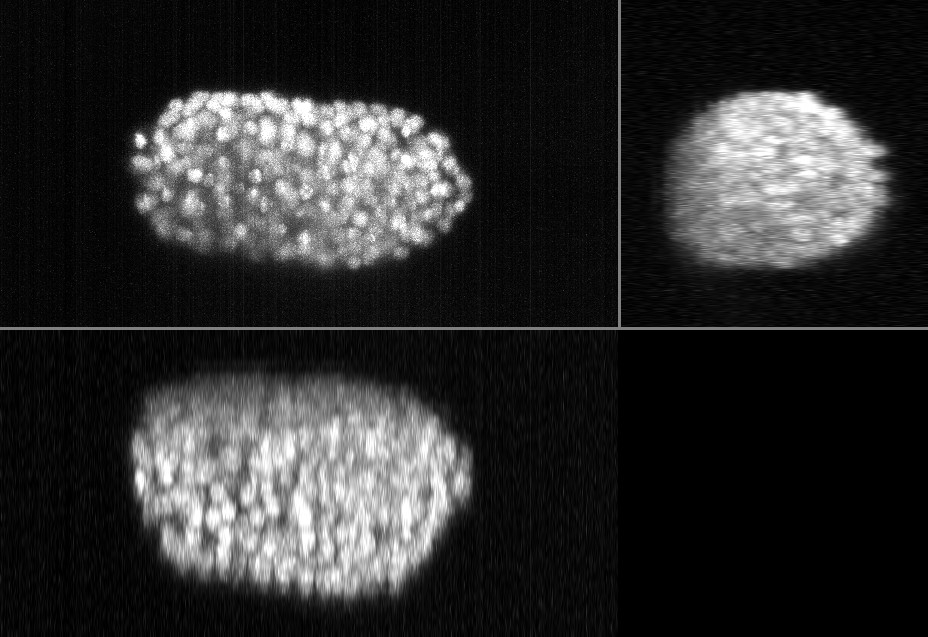
\includegraphics[width=\textwidth]{embryo2_T10_iso.jpg}
\caption{Reference: embryo\_2 early (T10)}
\end{subfigure}
\hfill
\begin{subfigure}[t]{0.45\textwidth}
\centering
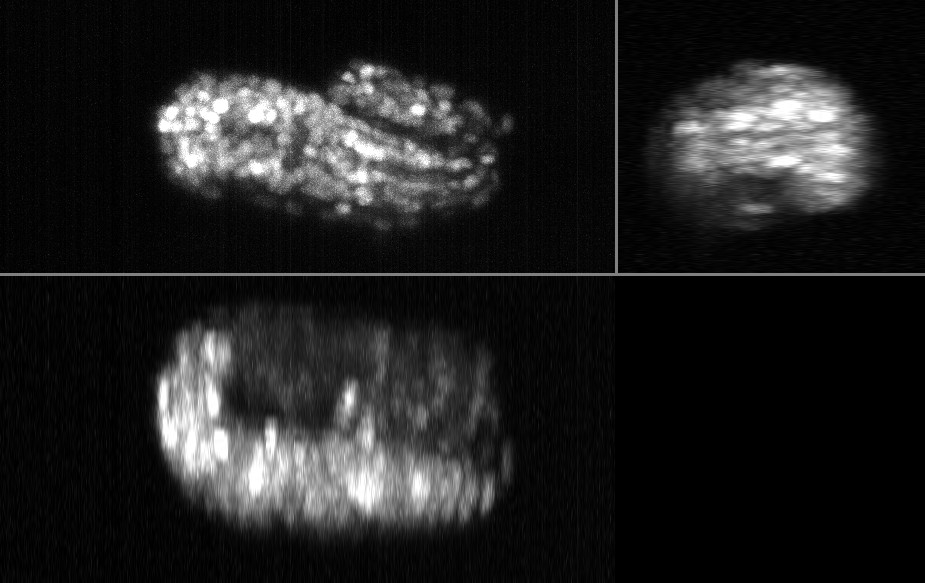
\includegraphics[width=\textwidth]{embryo2_T100_iso.jpg}
\caption{Reference: embryo\_2 pretzel (T100)}
\end{subfigure}

\vspace{8pt}

\begin{subfigure}[t]{0.45\textwidth}
\centering
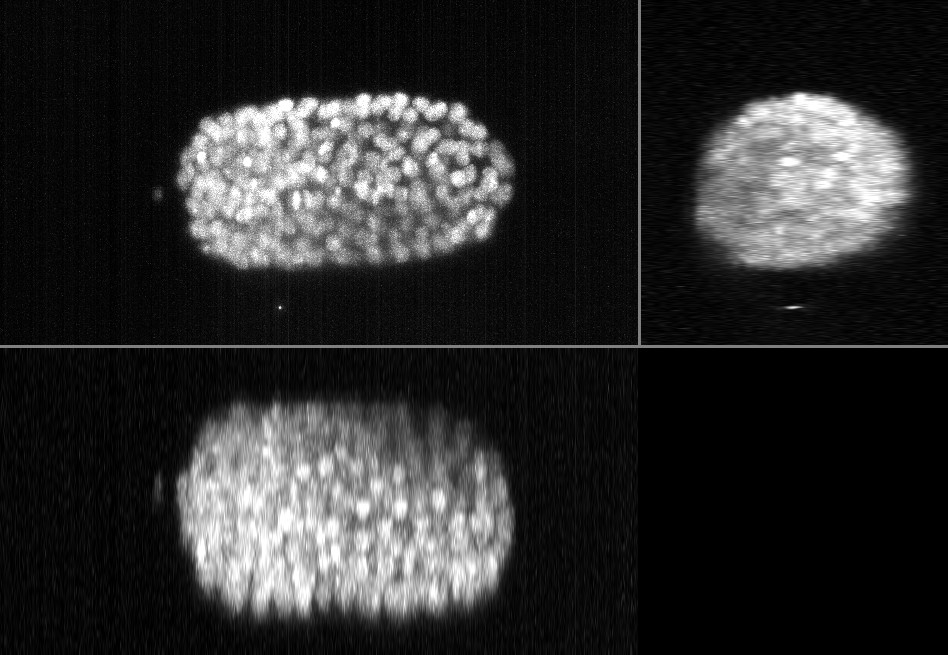
\includegraphics[width=\textwidth]{embryo3_T5_iso.jpg}
\caption{Embryo\_3 T5 (GT: early, predicted: pretzel)}
\end{subfigure}
\hfill
\begin{subfigure}[t]{0.45\textwidth}
\centering
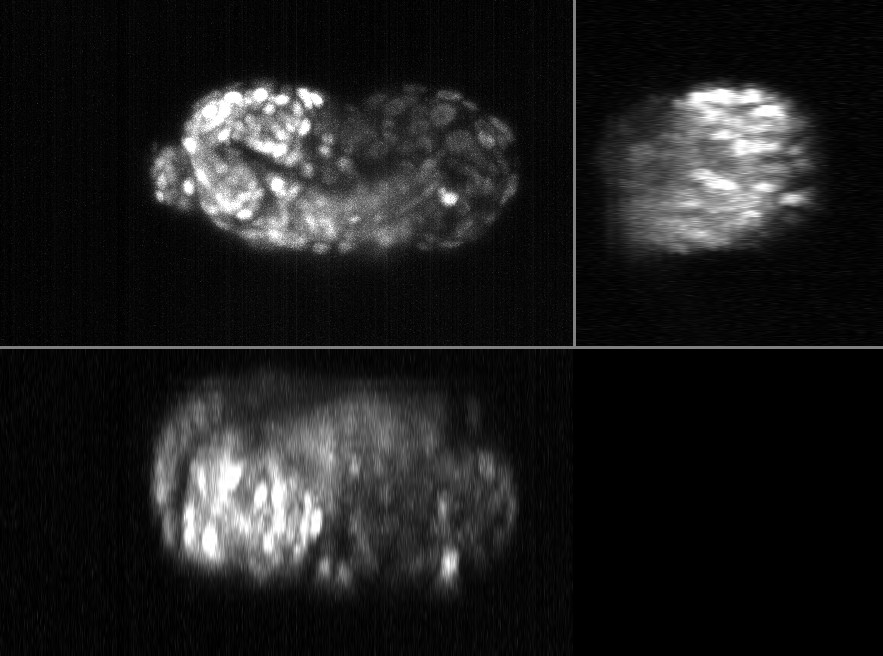
\includegraphics[width=\textwidth]{embryo4_T150_iso.jpg}
\caption{Embryo\_4 T150 (GT: pretzel, predicted: early)}
\end{subfigure}

\caption{Cross-stage confusion with isometric projection.  Top row: reference
images from embryo\_2.  Bottom left: embryo\_3 at early stage---its isometric
Z profile resembles the pretzel reference.  Bottom right: embryo\_4 at
pretzel stage---its Z profile does not match the pretzel reference, leading
to ``early'' predictions.}
\label{fig:confusion-case}
\end{figure}

% ═══════════════════════════════════════════════════════════════
\section{Methods}
% ═══════════════════════════════════════════════════════════════

\subsection{Isometric projection implementation}

The \texttt{projection\_three\_view()} function in \texttt{gently/imaging.py}
was modified to accept a \texttt{voxel\_size} parameter specifying physical
dimensions $(Z, Y, X)$.  When provided, the YZ and XZ projections are rescaled
along the Z axis by the ratio $Z_{\text{phys}} / XY_{\text{phys}}$ using
Lanczos interpolation.  The default was set to
$\texttt{voxel\_size} = (1.0, 0.1625, 0.1625)$, producing isometric output.

Resulting image sizes (typical):
\begin{center}
\begin{tabular}{@{}lrr@{}}
\toprule
\textbf{Projection} & \textbf{Non-isometric} & \textbf{Isometric} \\
\midrule
Three-view composite & $687 \times 385$ px & $944 \times 642$ px \\
Z-axis display height & $\sim$53 px & $\sim$310 px \\
\bottomrule
\end{tabular}
\end{center}

\subsection{Reference image regeneration}

All six stage reference images (\texttt{three\_view.jpg} in
\texttt{gently/examples/stages/\{early,bean,comma,1.5fold,2fold,pretzel\}/})
were regenerated from the benchmark source volumes (embryo\_2) using isometric
projection.  This ensures that both reference images and test images use
identical projection geometry---the model is not confused by a format mismatch.

No other reference files (e.g., \texttt{progression.jpg}) are loaded by the
\texttt{ExampleStore} when \texttt{three\_view.jpg} is present.  We verified
that only the \texttt{three\_view.jpg} files are sent to the model as reference
examples.

\subsection{Benchmark configuration}

\begin{center}
\begin{tabular}{@{}ll@{}}
\toprule
\textbf{Parameter} & \textbf{Value} \\
\midrule
Model           & \texttt{claude-sonnet-4-5-20250929} \\
Temperature     & 0.0 \\
Dataset         & Session \texttt{59799c78}, 4 embryos, 769 timepoints \\
Ground truth    & Manual annotation (Ryan Christensen, Dec 2024) \\
Reference images & 1 per stage (isometric \texttt{three\_view.jpg}) \\
Tools           & Disabled (single-pass classification) \\
Prompt caching  & Enabled (1h TTL on system prompt + references) \\
\bottomrule
\end{tabular}
\end{center}

Two prompt variants were tested:

\begin{enumerate}[leftmargin=*, itemsep=2pt]
  \item \textbf{Minimal:} Stage names and JSON output format only.
  \item \textbf{Descriptive:} One-line morphological description per stage
    (e.g., ``symmetric oval, dividing cells'' for early).
\end{enumerate}

Both variants include temporal context (last 3 predictions) and all 6 stage
reference images.

\subsection{Baselines}

The non-isometric baselines use identical prompt text, model, and dataset, but
with standard (Z-compressed) projections for both test images and reference
images.  These were run as part of the prompt ablation experiment
(Experiment~1 in the main benchmark plan).

% ═══════════════════════════════════════════════════════════════
\section{Results}
% ═══════════════════════════════════════════════════════════════

\subsection{Overall accuracy}

\begin{center}
\begin{tabular}{@{}lrrrl@{}}
\toprule
\textbf{Variant} & \textbf{Exact} & \textbf{Adjacent} & \textbf{$N$}
  & \textbf{$\Delta$ Exact} \\
\midrule
Minimal (baseline)       & 48.5\% & 65.4\% & 769 & --- \\
Isometric minimal        & 33.7\% & 49.3\% & 769
  & \textcolor{neg}{$-$14.8pp} \\
\addlinespace
Descriptive (baseline)   & 48.0\% & 65.1\% & 769 & --- \\
Isometric descriptive    & 40.2\% & 54.0\% & 769
  & \textcolor{neg}{$-$7.8pp} \\
\bottomrule
\end{tabular}
\end{center}

Isometric projections degrade accuracy in both variants.  The minimal prompt
is more severely affected ($-14.8$pp) than the descriptive prompt ($-7.8$pp),
suggesting that morphological text descriptions partially compensate for the
visual confusion introduced by isometric scaling.

\subsection{Per-stage accuracy}

\begin{center}
\small
\begin{tabular}{@{}l*{4}{r}@{}}
\toprule
& \multicolumn{2}{c}{\textbf{Minimal}} & \multicolumn{2}{c}{\textbf{Descriptive}} \\
\cmidrule(lr){2-3} \cmidrule(lr){4-5}
\textbf{Stage} & \textbf{Baseline} & \textbf{Isometric}
  & \textbf{Baseline} & \textbf{Isometric} \\
\midrule
early     & 98.1\% & 54.8\% & 98.1\% & 81.5\% \\
bean      & 75.0\% & 25.0\% & 45.8\% &  0.0\% \\
comma     & 22.2\% &  7.4\% & 55.6\% &  7.4\% \\
1.5-fold  & 12.2\% &  0.0\% & 18.4\% &  4.1\% \\
2-fold    & 82.3\% & 15.2\% & 45.6\% &  2.5\% \\
pretzel   & 28.6\% & 35.3\% & 33.3\% & 40.4\% \\
\bottomrule
\end{tabular}
\end{center}

Isometric projections cause catastrophic accuracy loss on intermediate stages
(bean through 2-fold).  Early stage accuracy drops from 98\% to 55--82\%.
Pretzel is the only stage that slightly \emph{improves} with isometric
projections (+6.7pp minimal, +7.1pp descriptive), likely because the
exaggerated Z dimension makes the tight coiling pattern more distinctive.

\subsection{Per-embryo accuracy}

\begin{center}
\small
\begin{tabular}{@{}l*{4}{r}@{}}
\toprule
& \multicolumn{2}{c}{\textbf{Minimal}} & \multicolumn{2}{c}{\textbf{Descriptive}} \\
\cmidrule(lr){2-3} \cmidrule(lr){4-5}
\textbf{Embryo} & \textbf{Baseline} & \textbf{Isometric}
  & \textbf{Baseline} & \textbf{Isometric} \\
\midrule
embryo\_1 & 37.3\% & 38.3\% & 57.5\% & 49.7\% \\
embryo\_2 & 50.5\% & 13.5\% & 43.2\% & 29.7\% \\
embryo\_3 & 37.5\% & 21.4\% & 22.9\% & 21.4\% \\
embryo\_4 & 68.8\% & 61.5\% & 68.2\% & 59.9\% \\
\bottomrule
\end{tabular}
\end{center}

The accuracy impact is highly non-uniform across embryos.  Embryo\_2 suffers
the most severe degradation (50.5\% $\to$ 13.5\% for minimal), while
embryo\_1 is essentially unchanged.  This is consistent with the hypothesis
that isometric scaling amplifies specimen-specific morphological features that
vary between embryos.

\subsection{Confusion patterns}

The isometric confusion matrices reveal a qualitatively different error pattern
compared to baselines (see Figures~\ref{fig:inter-embryo}
and~\ref{fig:confusion-case}).

\subsubsection{Baseline (non-isometric)}

Errors are predominantly \textbf{adjacent-stage}: the model predicts one stage
too early or too late.  The confusion matrix is nearly tridiagonal, with errors
concentrated on the off-diagonals.  This reflects genuine boundary ambiguity.

\subsubsection{Isometric}

Errors become \textbf{cross-stage}: predictions scatter across non-adjacent
stages.  Key pathological patterns:

\begin{itemize}[leftmargin=*, itemsep=2pt]
  \item \textbf{Embryo\_3, early $\to$ pretzel:} From T0, the model classifies
    early-stage timepoints as ``1.5fold'' or ``pretzel.''  The isometric side
    views of embryo\_3's early stage apparently resemble the reference pretzel
    image from embryo\_2 (Figure~\ref{fig:confusion-case}).

  \item \textbf{Embryo\_4, pretzel $\to$ early:} The reverse: late-stage
    timepoints are classified as ``early.''  The isometric Z profile of
    embryo\_4's pretzel stage does not match the reference pretzel (from
    embryo\_2).

  \item \textbf{Isometric minimal confusion matrix:} early stage predictions
    scatter to bean (21), comma (2), 1.5fold (6), 2fold (19), and pretzel (23).
    In the baseline, early predictions scatter only to bean (3).
\end{itemize}

\subsection{Calibration}

\begin{center}
\begin{tabular}{@{}lrrr@{}}
\toprule
\textbf{Variant} & \textbf{ECE} & \textbf{Conf (correct)} & \textbf{Conf (wrong)} \\
\midrule
Minimal (baseline)      & 0.424 & 0.901 & 0.920 \\
Isometric minimal       & 0.593 & 0.914 & 0.930 \\
\addlinespace
Descriptive (baseline)  & 0.422 & 0.901 & 0.907 \\
Isometric descriptive   & 0.509 & 0.891 & 0.934 \\
\bottomrule
\end{tabular}
\end{center}

Isometric projections worsen calibration.  The model is \emph{more} confident
when wrong than when correct (0.930 vs.\ 0.914 for isometric minimal), and
the ECE increases from 0.424 to 0.593.  The model does not recognize the
increased difficulty of isometric images.

% ═══════════════════════════════════════════════════════════════
\section{Analysis}
% ═══════════════════════════════════════════════════════════════

\subsection{Why isometric projections hurt}

The core finding is counter-intuitive: providing the model with physically
correct geometry \emph{reduces} classification accuracy.  We propose the
following explanation.

\subsubsection{Inter-specimen variation dominates inter-stage variation in Z}

Developmental stage classification relies primarily on features visible in the
XY plane: overall shape (oval, bean, comma), body folding, and coiling.  The Z
dimension carries relatively little stage-discriminative information.  What Z
\emph{does} carry is specimen-specific variation: each embryo sits at a
different orientation and depth in the imaging chamber.

With compressed Z (non-isometric), the side and front views are small and
contribute minimally to visual matching.  The XY (top-down) view dominates,
and stage-relevant features drive classification.

With isometric Z, the side and front views are $6\times$ taller and visually
prominent.  The model now gives substantial weight to the Z profile when
matching against reference images.  Since the Z profile varies more between
specimens than between stages, the model effectively performs
\textbf{specimen identification} rather than \textbf{stage classification}.

This explains the cross-stage confusion patterns: embryo\_3 looks like the
reference pretzel \emph{in Z}, regardless of its actual developmental stage
(Figure~\ref{fig:confusion-case}).

\subsubsection{Reference images are from a single specimen}

The reference \texttt{three\_view.jpg} images were generated from embryo\_2.
With non-isometric projections, the reference images are approximately
representative because the XY morphology (which dominates) is similar across
specimens at the same stage (Figure~\ref{fig:inter-embryo}, top row).  With
isometric projections, the reference images become specimen-specific:
embryo\_2's Z profile at each stage is now a prominent visual feature, and
other embryos with different Z profiles fail to match
(Figure~\ref{fig:inter-embryo}, bottom row).

\subsubsection{Descriptive prompt partially compensates}

The descriptive prompt includes text descriptions of morphological features
(e.g., ``body folding back on itself'' for 1.5-fold).  These descriptions
ground the model's classification in stage-relevant features rather than visual
template matching, partially offsetting the confusing Z-profile information.
This explains the smaller accuracy drop for the descriptive variant ($-7.8$pp
vs.\ $-14.8$pp for minimal).

\subsection{Implications for representation design}

This experiment provides an important design principle for projecting
anisotropic volumetric data for VLM classification:

\begin{quote}
\itshape
When the classification task depends on features in one set of dimensions (XY)
and specimen-level nuisance variation concentrates in another dimension (Z),
compressing the nuisance dimension is beneficial---even though it is physically
incorrect.
\end{quote}

The non-isometric projection acts as an implicit feature selection mechanism,
down-weighting Z-axis information that confuses rather than aids
classification.

% ═══════════════════════════════════════════════════════════════
\section{Conclusions}
% ═══════════════════════════════════════════════════════════════

\begin{enumerate}[leftmargin=*, itemsep=4pt]
  \item \textbf{Isometric projections are strictly worse} for VLM-based embryo
    stage classification: $-14.8$pp exact accuracy (minimal), $-7.8$pp
    (descriptive).

  \item \textbf{The Z axis carries more nuisance than signal} for this task.
    Physically correct Z-scaling amplifies inter-specimen variation that
    confuses visual template matching.

  \item \textbf{Text descriptions partially compensate} for visual confusion,
    suggesting that hybrid representations (images + structured text features)
    may be more robust than images alone.

  \item \textbf{Reference image diversity matters.}  Using reference images
    from a single specimen creates a representation bias that is masked by Z
    compression but exposed by isometric projection.  Multi-specimen reference
    sets may improve robustness for both projection types.

  \item \textbf{The default projection should remain non-isometric.}  The
    \texttt{projection\_three\_view()} function should not apply voxel size
    correction for perception tasks.  Isometric projection may still be
    valuable for human visualization or other analysis tasks where geometric
    accuracy matters.
\end{enumerate}

\subsection{Action items}

\begin{itemize}[leftmargin=*, itemsep=2pt]
  \item Revert \texttt{projection\_three\_view()} default to non-isometric
    (remove \texttt{voxel\_size} default).
  \item Restore reference \texttt{three\_view.jpg} images to non-isometric
    projection.
  \item Consider a future experiment with multi-specimen reference images to
    test whether reference diversity improves robustness.
\end{itemize}

% ═══════════════════════════════════════════════════════════════
\section*{Appendix: Raw Confusion Matrices}
% ═══════════════════════════════════════════════════════════════

\subsection*{A.1 Isometric Minimal}

\begin{center}
\small
\begin{tabular}{@{}l*{8}{r}@{}}
\toprule
& \multicolumn{8}{c}{\textbf{Predicted}} \\
\cmidrule(l){2-9}
\textbf{True} & early & bean & comma & 1.5f & 2f & pretzel & hatching & hatched \\
\midrule
early    & \textbf{86} & 21 & 2 & 6 & 19 & 23 & -- & -- \\
bean     & 6 & \textbf{6} & -- & -- & -- & 12 & -- & -- \\
comma    & 1 & 9 & \textbf{2} & 3 & -- & 12 & -- & -- \\
1.5-fold & -- & 8 & -- & \textbf{0} & 15 & 26 & -- & -- \\
2-fold   & -- & 3 & 2 & 2 & \textbf{12} & 60 & -- & -- \\
pretzel  & 201 & -- & -- & -- & -- & \textbf{153} & 4 & 75 \\
\bottomrule
\end{tabular}
\end{center}

\subsection*{A.2 Isometric Descriptive}

\begin{center}
\small
\begin{tabular}{@{}l*{8}{r}@{}}
\toprule
& \multicolumn{8}{c}{\textbf{Predicted}} \\
\cmidrule(l){2-9}
\textbf{True} & early & bean & comma & 1.5f & 2f & pretzel & hatching & hatched \\
\midrule
early    & \textbf{128} & 3 & 1 & 2 & 2 & 21 & -- & -- \\
bean     & 12 & \textbf{0} & 2 & 2 & 2 & 6 & -- & -- \\
comma    & 10 & 2 & \textbf{2} & 1 & 6 & 6 & -- & -- \\
1.5-fold & 8 & -- & -- & \textbf{2} & 13 & 26 & -- & -- \\
2-fold   & 3 & 2 & 2 & 4 & \textbf{2} & 66 & -- & -- \\
pretzel  & 31 & -- & -- & -- & -- & \textbf{175} & 3 & 224 \\
\bottomrule
\end{tabular}
\end{center}

\subsection*{A.3 Baseline Minimal (non-isometric, for comparison)}

\begin{center}
\small
\begin{tabular}{@{}l*{8}{r}@{}}
\toprule
& \multicolumn{8}{c}{\textbf{Predicted}} \\
\cmidrule(l){2-9}
\textbf{True} & early & bean & comma & 1.5f & 2f & pretzel & hatching & hatched \\
\midrule
early    & \textbf{154} & 3 & -- & -- & -- & -- & -- & -- \\
bean     & 5 & \textbf{18} & 1 & -- & -- & -- & -- & -- \\
comma    & -- & 15 & \textbf{6} & 2 & 4 & -- & -- & -- \\
1.5-fold & -- & 15 & 15 & \textbf{6} & 13 & -- & -- & -- \\
2-fold   & -- & -- & 7 & 7 & \textbf{65} & -- & -- & -- \\
pretzel  & 186 & -- & -- & -- & 69 & \textbf{124} & -- & 54 \\
\bottomrule
\end{tabular}
\end{center}

\end{document}
